
\section{IME Architecture}
IME system is based on a Client-Server interaction: every compute node has a
Client side process intercepting IO communications that are sent to IME servers.
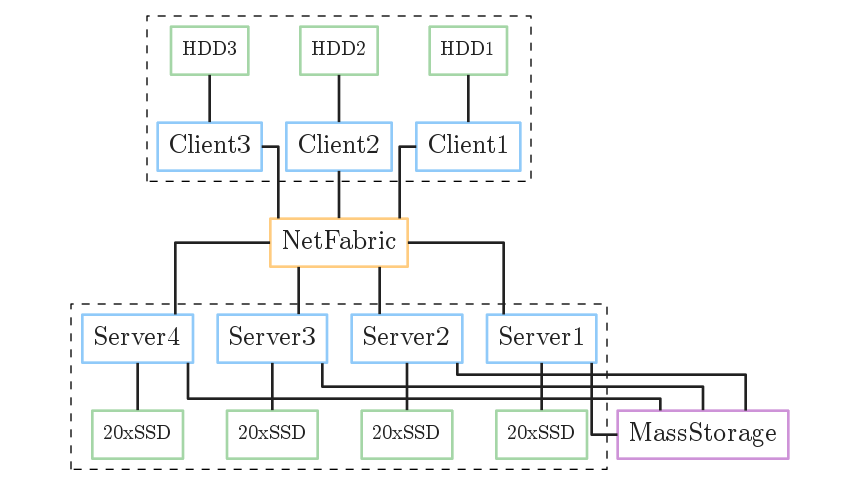
\includegraphics[width=\textwidth]{map.png}
The picture capture a possible configuration of IME:
\begin{itemize}
    \item 3 Clients with a single HDD each. These will generate the data that
        has to be stored in IME servers.
    \item a Network Fabric that interconnects every component of IME
    \item 2 SSDs per server, that can store data faster compared to the single
        client's HDD
\end{itemize}

Given the skeleton of the architecture, can be added or removed clients,
servers and disks for each one. This changes will end in different performances
that the simulator must be able to detect. \\
Part of the work is to inspect also different system layouts. The advantage of a
simulator is the ability to ensure the quality of a layout without the need to
test it for real, assuming the simulator is precise enough.
Every layout will be discussed in depth in the analysis section
(\ref{sys-analysis}).

\subsection{Network communication time}\label{netbuff}
Network communication is one of the main task that are committed in this system,
so we need an accurate model to represent it. \\
The parameters that determine the time elapsed in a network transaction are
\textit{latency} and \textit{bandwidth}. A file in theory is sent dividing
its size by the bandwidth available. In the real world we have to keep account also
the latency present inside the system: the smallest file will be sent
only after $<latency>$ amount of time. \\
From \cite{packet-size-ib} we know that the optimal packet size for
communication over infiniband is 1MB. \\
IME Client packs together requests smaller than this threshold and split bigger
files to achieve this communication pattern. This is further referred as
\textbf{Network Buffer}.  If requested explicitly, every request can be flushed
in order to complete a communication in case of remainders.  This set a domain
over the size of the packet sent: we always will have packets that are in the
interval $]0, 1024] KB$. The model should predict correctly the time required by
any network communication inside this interval. \\ In this case the only bond I
have are the 2 coordinates \\

\vspace{0.5cm}
\begin{tabular}{c | c}
    file size (KB) & time required \\ \hline
    0 & \textit{latency} \\ \hline
    1024 & \textit{1024KB / bandwidth}
\end{tabular}
\vspace{0.5cm}

These are respectively the worst and the best usage of the network. \\
I can obtain a more accurate model running some benchmarks on IME network, but
from a starting point I can rely on these 2 constraint. \\
Having the possibility to choose my interpolating function, I decided to use a
function with a diagonal limit, namely $\lim_{x \to +\infty} y(x) = +\infty$,
that is a real behaviour for every network. \\
The function of choice then is an \textit{hyperbole} adjusted to match the
specified coordinates. \\
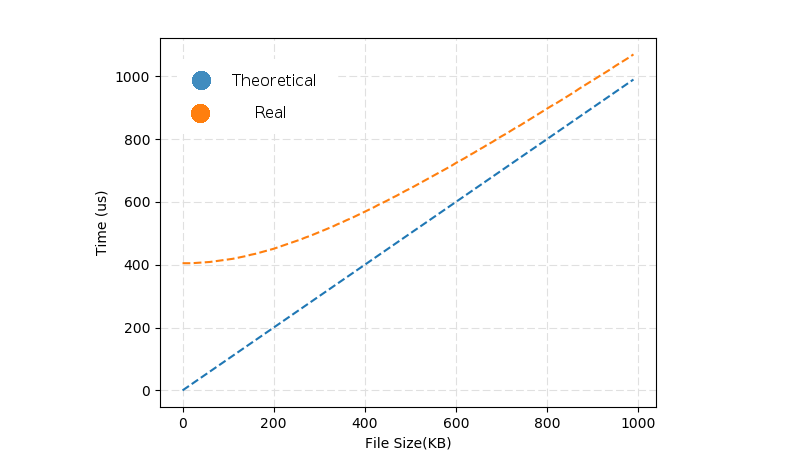
\includegraphics[width=\textwidth]{diaglimit.png}


\subsection{Tokenized communication}
IME has been designed to be employed with a large number of both clients and
servers. This lead to many parallelization problems and resource management.
With a large amount of clients, the network bandwidth will run out very quickly.
To overcome this problem, the client side of IME is based on a Tokenized Network
Communication. The concept of the token is similar to the Token Ring
communication \cite{token-ring} that prevents a single client to use all the
resources of the system and sharing equally the bandwidth among all the
clients.  Here instead of having a single token shared over all the clients,
each client has a fixed amount of tokens.\\
The token usage is the following:
\begin{itemize}
    \item Consumed when making a request
    \item Recovered when receiving an answer
\end{itemize}
This means that for \textit{n} token, a single client can have \textit{n}
communications in parallel.  So far DDN already set a value of 24 tokens that
are not completely used in real applications, meansing that there is not a
bottleneck, but is anyway a free parameter that can be inspected and adapted in
the simulator.


\subsection{Erasure coding for data loss} \label{pargroup}
In CPU caches, whenever happens a cache miss, data is read from main memory
instead. No data can be potentially lost. In the worst case cache won't be
useful. \\
IME acts as a cache too but for the problem it is solving, there is no
communication between the source and the target. This means that if data
is lost inside IME, it is \textit{permanently} lost. IME has a system to
overcome this problem that is \textit{Erasure Coding}. \\
As it happens in RAID level 4, 5 and 6, what is stored in the disks is not just
data but also an added amount of data based on the original data. In case of
loss of one piece of data, this missing part can be reconstructed comparing
remaining data and parity. \\
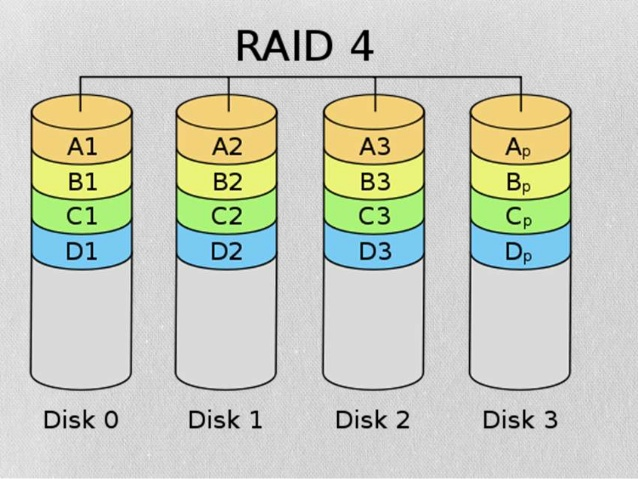
\includegraphics[width=\textwidth]{raid-level4.jpg} \\
For this correction system to work, we need to make associations between groups
of data that must be grouped together later when data loss happens. IME
considers a single block of data a Network Buffer (see \ref{netbuff}) and the
group that will contribute to data recovery as a \textbf{Parity Group}. \\
As an example, from the picture A1, A2, A3 and A$_p$ are individually a Network
Buffer. All of them grouped together makes a Parity Group. \\
The parity is generated by the client since the servers has only to keep track
about their status. \\
Is essential that every piece of the same parity group are sent to
different server: the loss of a single server could otherwise means the loss of
multiple piece of data. If every part is stored in a different server, the
inactivity of a single machine is not a fatal error for the system.

\subsubsection*{Handling remainders}
Using this system to recover data, a bond is created among parts of the same parity group:
no only these parts share the same group-id but also must be sent at the same time so servers,
otherwise inconsistency are created sending to server a parity group that cannot be completely gathered
and so rebuilt in case of data loss. \\
Client must wait until is has enough data to send, filling a set of network buffers. If it does not have
enough data, it waits until more write requests are performed. The send operation can anyway be forced using an
\textbf{eager commit}, sending buffers not completely filled or even not enough buffers to fill a parity group. \\
Parity data is then generated using the data available.

\newpage
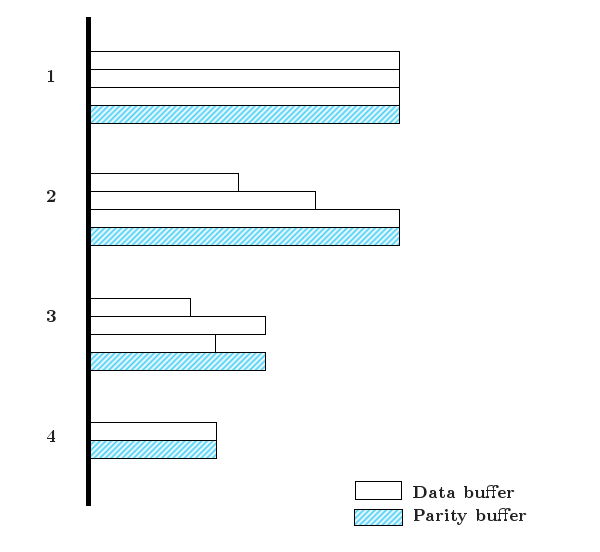
\includegraphics[width=\textwidth]{parity-remainder.png}
The upper image shows the parity distribution with geometry 3+1.
\begin{enumerate}
    \item Canonical case: every buffer is sent and parity is generated base on every buffer
    \item Only a buffer reaches its maximum size and parity is generated based on the biggest buffer,
        considering zeros for the other missing data
    \item None of the buffers reachs its maximum size, so parity is based on the biggest one
    \item There are not enough buffers to fill the group and parity is generated based always
        on the biggest buffer.
\end{enumerate}

\subsection{File queuing}
Every clients has internally a write queue for every single server. As it is
asked to write a file, the client will scatter the single file to multiple
queues in order to make us of most servers and speed up the transaction.
When a client wants to perform a write it has to care about:
\begin{itemize}
    \item The amount of servers that will be involved depending on the file size
    \item Not scattering too much a single file to avoid unnecessary broadcast
        operations reading a small amount of data
    \item Perform small transactions of 1MB to maximize network bandwidth
\end{itemize}
Since this system involves not only disk operations but also network ones, we
must be careful to not deplete the network resources. This means that to
maximize an IO operation, make sense using as many devices as possible, but in
a network environment is better to reduce at minimum the packets emitted. \\ To
overcome these opposing behaviour, IME has 2 layers of file queuing:
\textbf{bucket}-based and \textbf{buffer}-based queuing systems.  A bucket is
considered as a part of a file of a fixed size. A single file is split in
bucket-sized parts and then queued to be split again to buffer-sized parts, in
order to perform a network communication.
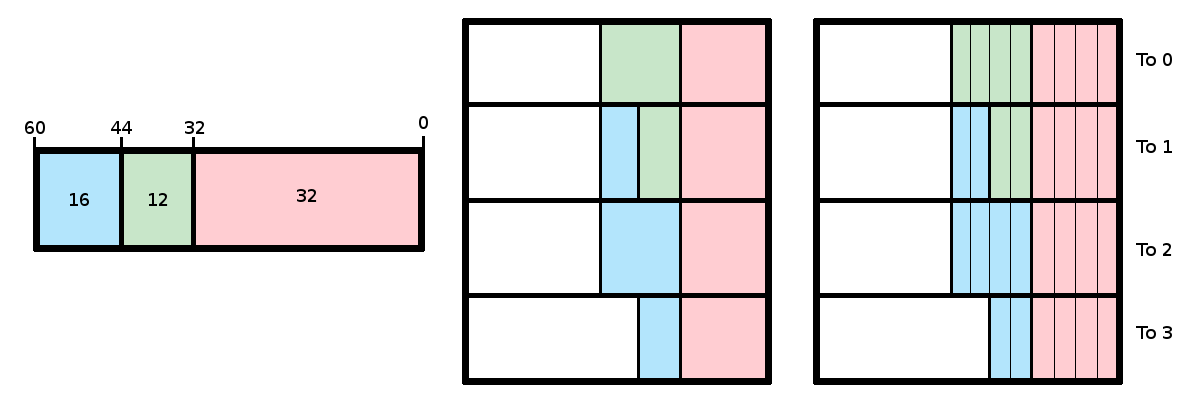
\includegraphics[width=\textwidth]{queuing.png}
\begin{itemize}
    \item 4 servers are installed
    \item the user asked to write every file, 32, 12, 16 MB respectively, in
        chronological order.
    \item Bucket size = 8MB
    \item Buffer size = 2MB, just for plotting purposes
    \item parity is not considered
\end{itemize}
In the upper picture the first queue is the file-oriented one: every file as it seen
by the client point of view.  Then the central box represents the queue to each
server with the bucket view of the files.  The last one represents also the
server's queues but with network buffers instead of buckets. \\ This different
granularity allows to make us of the server's devices if a file is big enough,
saving at the same time network operations when the user asks to read those
later.\\
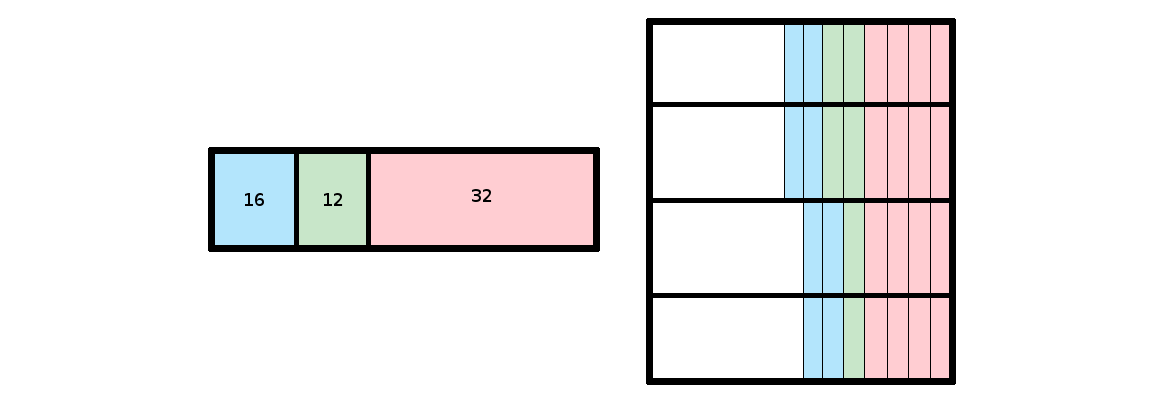
\includegraphics[width=\textwidth]{queuing-nobuckets.png}
The upper image shows how packets should be distributed without the bucket queuing layer.
Note that, from the buffer point of view, the green file could be
split over all the servers, that translates in great write operation but poor
read operation, since it has to perform a broadcast over all the system. This
example must be thought with bigger numbers: in a case with 50 servers, with a
buffer point of view, a file of 50MB involves a broadcast, while the bucket
point of view mitigate this behaviour increasing the file size required by a
broadcast to 400 MB. \\
Some examples in the following table shows the \textit{number of read requests generated}
from a single client reading a file, using the bucket view or not where 50 servers are installed.

\vspace{0.5cm}
\begin{tabular}{l | c | c}
    & \multicolumn{2}{|c}{Number of requests using} \\
    Data read & also buckets & only buffers \\ \hline
    1 MB & 1,2 & 1,2 \\
    8 MB & 1,2 & 8,9 \\
    48 MB& 6,7 & 48,49 \\
    400 MB & 50 & 50 \\
\end{tabular}
\vspace{0.5cm}

For requests size below 400MB there are benefits reducing the number of read
requests generated and so the netowork traffic. For requests bigger than 400MB
we cannot see the difference since network traffic reduction has been overcome
by IO operations.

\subsubsection*{HDD behaviour}\label{hdd-behaviour}
There is a lower minimum size an HDD interact with. If the user wants to edit a
single byte on the file system, the HDD will read a bigger amount of data,
accept user modification, and write again the bigger amount of data. If this
amount of data is 256KB, for instance, performing 8 write of 256KB or 1B each,
will result in the same performances.  The only difference is that, if we are
aware of this fact, we can make use of it writing 2MB instead of 8B
respectively.

\subsection{Distributed Hash Table (DHT)}
IME servers must be aware of the data that are inside the system, being also
fault tolerant in case of failures. These should also be careful of not flooding
the network with too many requests. \\
DDN used a DHT to solve this problem, allowing the scaling of the number of
servers and allowing the failure of a single one. \\
As a file is stored to a server, its metadata, its way to access it are sent to
another server responsible of delivering the accidentally lost data.

\subsection{Server side write}
As the server receive a buffer, a number of steps are performed before sending
back an ack to the client. \\ Two separate task are performed, divided in 2
different planes: \textbf{Control plane} and \textbf{Data plane}

\subsubsection*{Control plane}
Here is performed metadata propagation if necessary and done some
\textit{logging} operation to a local journal device. \\ Metadata propagation
involve the communication of the current metadata to another machine, meaning
that this operation has to wait an ack before being completed.  This can hit
very hard the performances, forcing an additional network communication for
every write. So this operation is cached instead and done as one of the
following condition is met:
\begin{itemize}
    \item Client requested an eager commit
    \item Cache limit reached. After 128 requests is sent a single request
        instead of 128
    \item Timeout triggered. If no write happened recently, current
        data must anyway be saved so is forced a propagation
\end{itemize}
Metadata propagation is a necessary step in order to recover data in case of
failures: the medatata can be read from the DHT of another working server, then
data can be recovered asking to every involved server the lost parity groups.

\subsubsection*{Data plane}
Data received is stored locally as well as metadata. Since data and metadata
are accessed in a different pattern, and metadata represent a bottleneck when
it comes to files reading, metadata are stored in dedicated devices, less
capable but with wider bandwidth. \\
The problem to face in this case is to make use of every device understanding
the way every device works. \\
As for network communications, the diagonal limit behaviour (see section
\ref{netbuff}) can be applied also in this case. Then we look for bigger
transactions, avoiding small ones. \\
The request is seen in a twofold way: \\
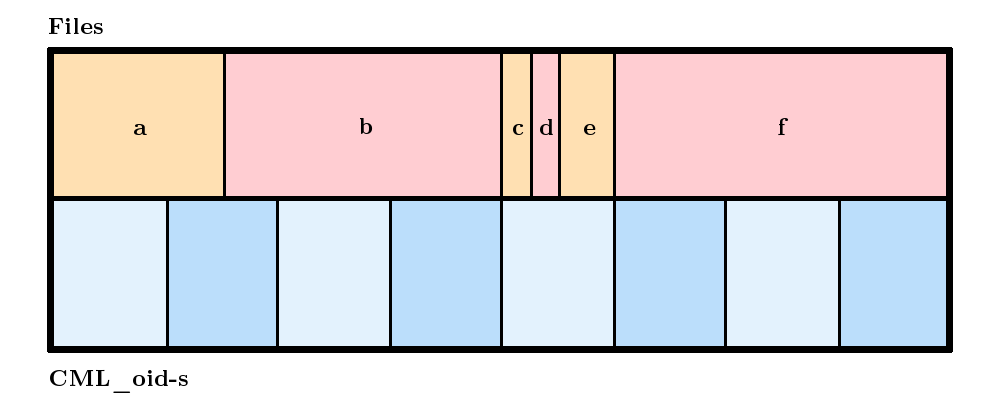
\includegraphics[width=\textwidth]{cmloid.png}
\begin{itemize}
    \item As a set of file parts. These informations are stored as metadata, in
        order to know exactly where each file part is stored. In the picture
        this is represented by the upper layer. In this case the user sent files
        \textit{a,b,c,d,e} and \textit{f}
    \item As a byte stream: aware of the behaviour of HDD (see section
        \ref{hdd-behaviour}) we are now interested in the data as a set of bytes
        to be written to the disk, nothing more. Metadata will tell us the exact
        location of a file, but we know want to perform the most efficient
        operation. \\
        In this step the network is split in \textbf{CML\_oid}s, chunk of 128KB.
        Each of these will be stored to different device, if possibile, in a
        round-robin fashion to distribute equally the load. \\
        In the picture the CML\_oid-s generated are the light blue boxes
\end{itemize}

\subsection{Data Read}
If a client wants to read a file, or a part of it, it interrogates its file map
to make a request to the interested server, saving netowork communication
avoiding a broadcast if not necessary. \\
After the server received the request, it has to interrogate its local DHT in
order to know from which devices has the requested data. A read operation is
then performed on those devices and data is sent back to client using as always
a buffered communication of 1 MB per packet. \\
This is the optimal workflow, that is without any kind of error.

\subsection{Data Recovery}
This is the case when a device cannot read anymore from one of its devices, for
any kind of reason. The server is now unable to satisfy the client's requests
and has to recover the data lost using the Erasure Coding system. \\
In case the server has lost also its metadata, it has to recover it from the
responsible server in the DHT. After this is recovered it has to gather al the
buffers involved in the lost parity groups. This is a very expensive operation
that can stop the system for a while but prevents the total interruption of the
service. \\
After every buffer of a parity group is retrieved, the missing buffer can be
regenerated using the parity information. If has been lost a parity buffer,
recovery is anyway necessary to prevent future failures.

\subsection{IO operations}
IME supports different IO operations depending on the task
\begin{itemize}
    \item \textbf{Sync}: the content of IME is copied to the mass storage, in
        order to have 2 copies of it. \\
        An use case can be keeping a remote file consistent to be read from
        others server later, leaving the chance to edit it later on IME.
    \item \textbf{Purge}: the files on IME are moved to the mass storage, not
        leaving any data on IME server. \\
        An use case is making some space because the disk is too filled, making
        space for some other data.
    \item \textbf{Erase}: files on IME are deleted, not making more copies of
        them. \\
        Happens when the data stored are just temporary, so there is no need to
        propagate further in the system.
\end{itemize}

These operations will be implemented in the simulator as well in order to better
classify the models. The objective is to test a model against a set of these
operations and extracting some measure to classify it.
